\Th \textbf{Теория Кумера}: $K \supset F$ - расширение Галуа, причём в $F$ лежат все корни n-ой степени из 1; $[K : F] = n$. Тогда $K$ циклическое $\Leftrightarrow$ $K$ - поле разложения для какого-то $x^n - a$, $a \in F$

\Proof 
$\Leftarrow$: доказано.

$\Rightarrow$: $Aut_F K = < \sigma > $ - циклическая; $\xi_n$ - примитивный корень n-ой степени из 1. Если всё хорошо, то для искомого $a$ верно $\sigma(a) = \xi_n a, \sigma^k(a) = \xi^k_n a, \sigma^n(a) = a, \sigma(a^n) = a^n$

$(1 + \xi_n \sigma + \xi_n^2 \sigma^2 + \dots + \xi_n^{n-1} \sigma^{n-1})(\beta) = \theta$

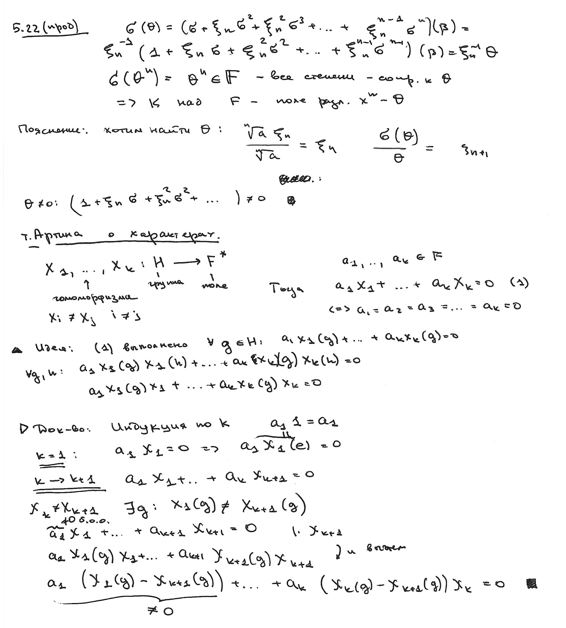
\includegraphics[]{images/5_22.JPG}